\documentclass[12pt]{article}
\usepackage{xr,geometry,fancyhdr,ifpdf,amsmath,paunits,smallsec}
\usepackage{color,lastpage,longtable,url,float,shortcuts}
\geometry{letterpaper,top=50pt,hmargin={20mm,20mm},headheight=15pt} 

\pagestyle{fancy} 
\fancypagestyle{first}{
\lhead{\textbf{A301}}
\chead{Doppler summary} 
\rhead{p.~\thepage/\pageref{LastPage}}
\lfoot{} 
\cfoot{} 
\rfoot{}
}

\ifpdf
    \usepackage[pdftex]{graphicx} 
    \pdfcompresslevel=0
    \DeclareGraphicsExtensions{.pdf,.jpg,.mps,.png}
    \usepackage{hyperref}
\else
    \usepackage{hyperref}
    \usepackage[dvips]{graphicx}
    \DeclareGraphicsRule{.eps.gz}{eps}{.eps.bb}{`gzip -d #1}
    \DeclareGraphicsExtensions{.eps,.eps.gz}
\fi

\newcommand{\rad}{%
   \ensuremath{I}
}

\newcommand{\irrad}{%
   \ensuremath{F}
}


\newcommand{\zenith}{%
   \ensuremath{\theta}
}

\newcommand{\azimuth}{%
   \ensuremath{\phi}
}

\newcommand{\optd}{%
   \ensuremath{\tau}\xspace
}


\newcommand{\trans}{%
   \ensuremath{Tr}
}

\newcommand{\abs}{%
   \ensuremath{\alpha}
}


\newcommand{\volabs}{%
   \ensuremath{\sigma}
}

\newcommand{\massabs}{%
   \ensuremath{\kappa}
}

\graphicspath{{./figures_tex/}}

\begin{document}
\pagestyle{first}

\begin{center}
ATSC 301:  Doppler notes\\
\end{center}


\noindent

\section{Doppler equations}
\label{sec:changes}


\begin{itemize}
\item First year physics:
\par
A stationary observer watching ripples go by with wavelength $\lambda$
and speed $c$ for a time $t$ will see

\begin{equation}
  \label{eq:rip1}
\mathrm{stationary\ wave\ count}=\frac{ c t}{\lambda}
\end{equation}
waves go by.

If the target begins to move towards the observer at speed $M_r$,
defined as negative when the distance between the target and observer
decreases,
then, compared with a measurement from a stationary target,
the observer will see more wave peaks over the same time.  The
additional number of peaks encountered during time $t$ is:

\begin{equation}
  \label{eq:rip2}
  \mathrm{additional\ crests}=\frac{ -M_r t }{\lambda}
\end{equation}

Alternatively, suppose we are in a boat moving towards  waves at speed $-M_r$,
while the waves are themselves moving towards us at speed $c$.
Since we are moving, we will hit more peaks than if we stayed still and
let the waves wash by us.  To find the frequency at which we're bobbing
up and down, just divide the number of peaks we encounter
by the time $t$:

\begin{equation}
  \label{eq:rip3}
  f_r = \frac{\frac{ct }{\lambda} + \frac{-M_r t }{\lambda} }{t} = f_t + f_{d}
\end{equation}



\item The round-trip effect
\par
Comparing  Stull equation 8.32 shows that there's a factor
of two missing from $f_d$ in (\ref{eq:rip3}).  That's because equation
(\ref{eq:rip3}) was derived for an observer moving towards an
oncoming set of waves.  In the case of radar the source and observer are at the
same point, and the waves are traveling to the cloud and returning.  Suppose
the cloud is $r$ km away, and in time t that 
distance to the cloud decreases  to $r - \Delta r$.  Then the roundtrip distance the
radar pulse has to travel changes from $d_0 = 2r$ to
$d_1=2r - 2 \Delta r$.  This round trip distance is what
causes a change in the waves reaching the receiver. So we need
to rewrite~(\ref{eq:rip2}) as

\begin{equation}
  \label{eq:rip4}
  \mathrm{additional\ crests}=\frac{(d_0 - d_1) }{\lambda}
  =\frac{2 \Delta r }{\lambda} =  \frac{-2 M_r t }{\lambda}
\end{equation}

Note that we have defined $M_r = \frac{dr}{dt}$ as \textbf{negative for velocity towards the radar}.
That is, a positive phase shift happens when the length $r$ between the radar and the target
is growing smaller.

Note that there is also a phase shift that happens when the wave goes from a medium with
low refractive index (air), to one with high refractive index (liquid water).  In that case
even a stationary target produces a positive phase shift of $\phi = \pi$.  (Going the other
direction, from water back to air, produces no phase shift).   

As shown in the reflection graph below.

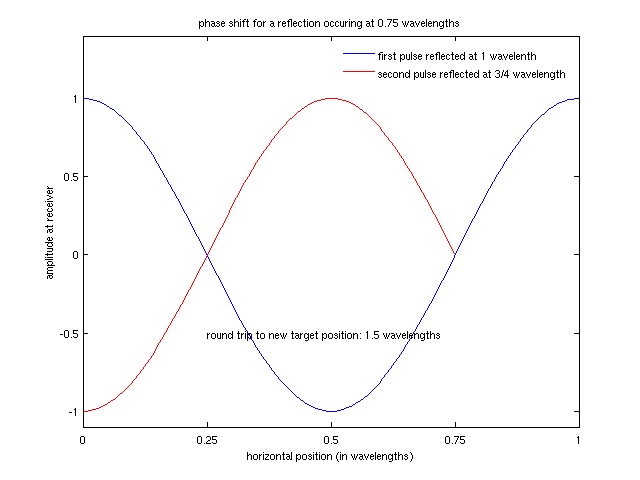
\includegraphics[width=0.6\textwidth]{figures_tex/reflection.png}


How do we know that the phase shift is positive?  The next figure
 shows a plot of:

\begin{equation*}
  A(x) = \sin(ft + \phi)
\end{equation*}
where the phase shift $\phi$ is 30, 60, 90, $\ldots$ degrees;

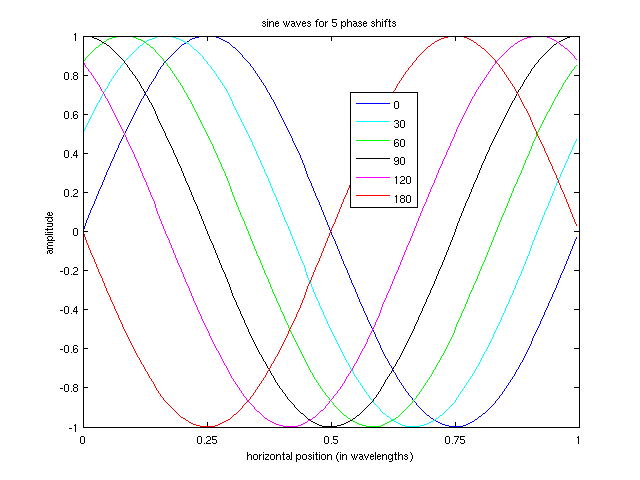
\includegraphics[width=0.6\textwidth]{figures_tex/sine_waves.png}

as the phase increase from blue to cyan to green, etc., the
wave appears to be traveling to the left, back to the radar.

Here is what the phase shift looks like on a phasor plot:


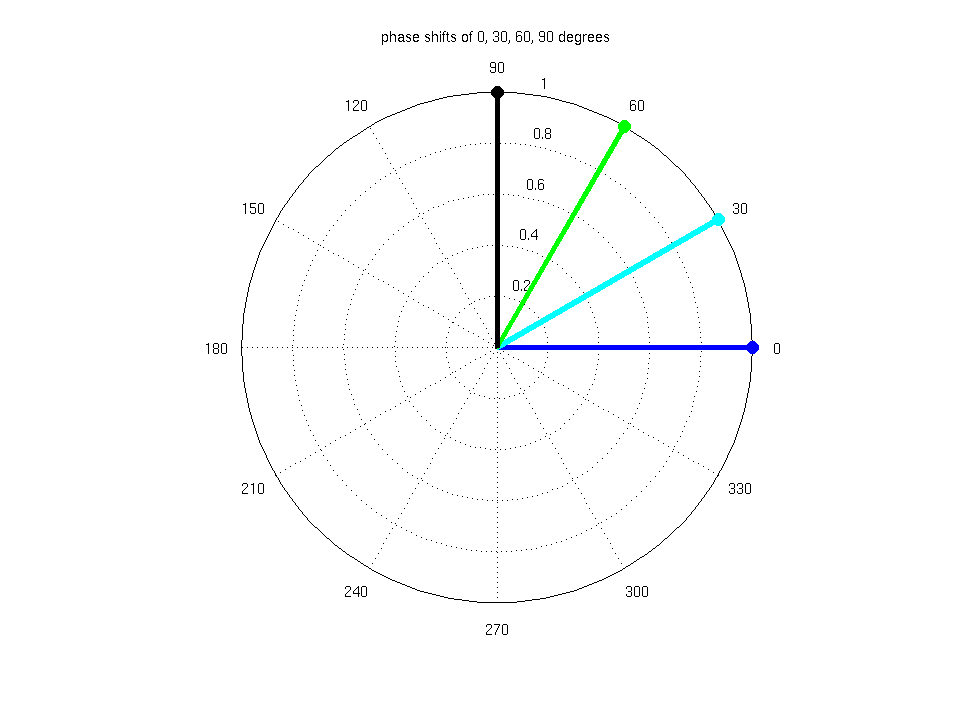
\includegraphics[width=0.6\textwidth]{figures_tex/polar_phase.png}

And you should convince yourself that at the radar:

\begin{equation*}
  A(t) = \cos(ft + \phi)
\end{equation*}
agrees with the phasor diagram:

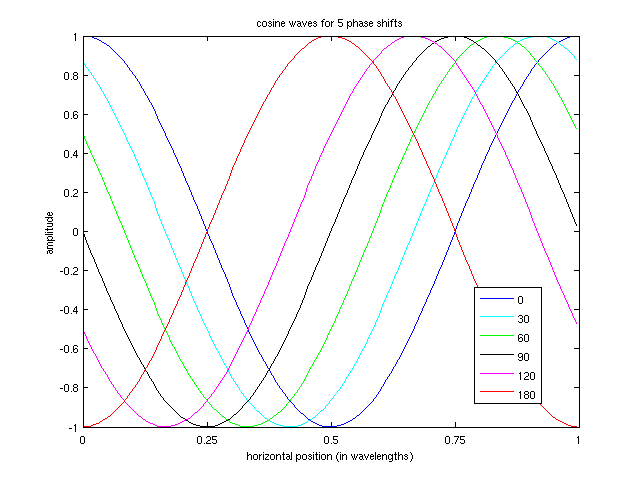
\includegraphics[width=0.6\textwidth]{figures_tex/cosine_waves.png}



 With the new (\ref{eq:rip4}),


\begin{equation}
  \label{eq:rip5}
  f_r = \frac{\frac{ct }{\lambda} + \frac{-2 M_r t }{\lambda} }{t} = f_t + f_{d}
\end{equation}
producing a doppler frequency of $f_d= -2 M_r/\lambda$ as expected.  (again, we're
defining $M_r$ as negative into the radar).

\item What is the maximum unambiguous velocity for a $\lambda$=10 cm radar
with a PRF of 400 Hz?
\par
\begin{itemize}
\item Note that we must make at least two observations per wavelength
(sample the wave at twice its frequency) to avoid aliasing.  


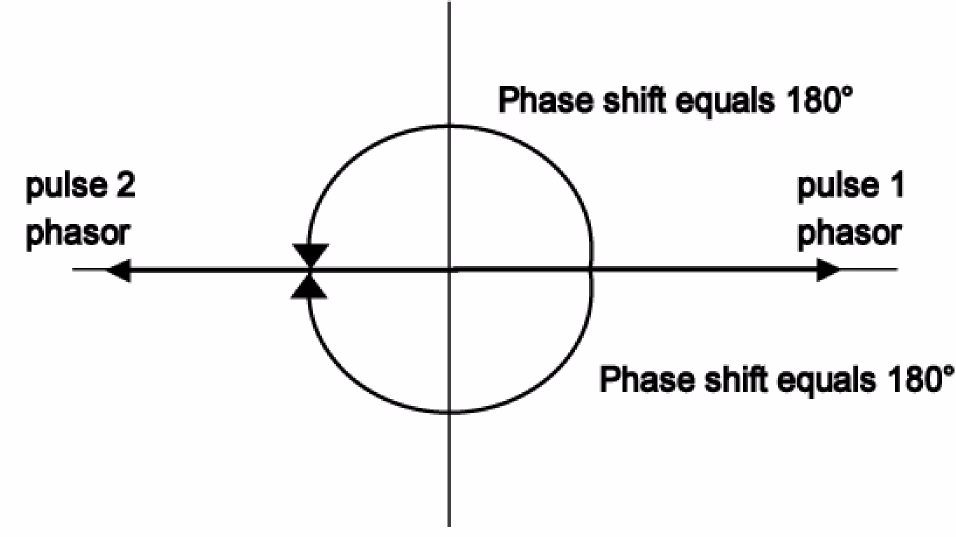
\includegraphics[width=0.6\textwidth]{figures_tex/alias.png}

To the radar a phase shift of +181 degrees and -179 degrees 
are indistinguishable for the same reason that to resolve a wave
you have to have at least two samples.  The +181 phase shift
into the radar is \textit{aliased on} (mistaken for) a 
-179 degree phase shift away from the radar.


\end{itemize}

So what is the phase shift between two pulses as a fraction of
wavelength? It's

\begin{equation}
  \label{eq:phi1}
  \frac{ \phi_2 - \phi_1}{2 \pi}
\end{equation}
This is the phase angle that builds up between two pulses due
to the fact that one pulse is shifted to a different frequency,
That is

\begin{equation}
  \label{eq:phi1}
  \frac{ \phi_2 - \phi_1}{2 \pi} = T_r f_d = 2 T_r M_r/\lambda
\end{equation}
where $T_r = 1/PRF$ is the time between pulses.  $\phi_2$ is bigger
than $\phi_1$ if $f_d > 0$, because the phasor will spin through
a large counterclockwise angle at the higher doppler-shifted
frequency.

And what is the displacement of the wave at the receiver as
a fraction of the wavelength due to the target moving a distance
$d$?  It's  $\frac{ 2d}{\lambda}$.
But we also know that:

\begin{equation}
  \label{eq:dpulse}
  d=T_r \times -M_r = -M_r/PRF
\end{equation}
where $M_r$ is the
radial target velocity  \textbf{defined as negative towards the radar}.  Equating these two representations of
the phase shift:

\begin{equation}
  \label{eq:phi2}
  \frac{ \phi_2 - \phi_1}{2 \pi} = \frac{2d }{\lambda}
= \frac{-2 T_r M_r }{\lambda} = \frac{ -2M_r}{\lambda PRF}
\end{equation}

Where we've used the round trip displacement of $2d$.

Finally, recognizing that the biggest phase shift we will be
able to measure in one half wavelength, which is 
$\phi_2 - \phi_1 = \pi$.  With this (\ref{eq:phi2})
becomes:

\begin{equation}
  \label{eq:phi3}
  \frac{ \pi}{2 \pi} =  \frac{ 2M_{r max}}{\lambda PRF}
\end{equation}
or 
\begin{equation}
  \label{eq:phi4}
M_{r max} = \frac{\lambda PRF }{4} = \frac{0.1 \times 400 }{4} = 10\ \ms
\end{equation}
for $\lambda$=10 cm and PRF=400 Hz.
\end{itemize}
this is Stull 8.35.  See also Stull Figure 8.35.

Stull pp. 251 talks about the ``doppler dilemma''.
This is the sad fact that to get the maximum range you need
 a low PRF, and to get the maximum unambiguous velocity you need
a high PRF:

\begin{equation}
  \label{eq:rmax}
  R_{max} = \frac{c }{2 PRF}
\end{equation}
and
\begin{equation}
  \label{eq:vmax}
  M_{rmax} = \frac{\lambda PRF }{4}
\end{equation}
so that
\begin{equation}
  \label{eq:total}
  R_{max} M_{rmax} = \frac{c \lambda }{8}
\end{equation}

\textbf{Summary: }  The factor of 1/4 in (\ref{eq:vmax}) arises from two factors
of 1/2:  one from the round trip displacement, and one from the requirement that
we not alias the velocity.  We can get better resolution of both range and velocity
by using longer wavelengths, but that means bigger antennas.


\section{Another perspective -- matching Stull eq. 8.32}
\label{sec:another-perspective}

Look at this from the point of view of wavelength.  Suppose
we have wavespeed $c$ and frequency $\nu$ (where I've changed
from $f$ to $\nu$ to match Roland), so that the wavelength
$\lambda = \frac{ c}{\nu}$.   If the waves are reflecting off
of a target that is a distance $r$ away then it takes them
$t=2r/c$ seconds to get back to the receiver, and in that
time the source produces $\nu t$ new waves, so there are always
$\nu t=\frac{\nu 2r }{c} = \frac{ 2r}{\lambda}$ waves between
the radar and the target.  But what if the target starts moving
towards the receiver?  Now the waves have to fit into a
shrinking distance, so the average wavelength is going to
decrease.  How much less room is availble?  Every cycle the
distance shrinks by $\frac{2 }{\nu} \frac{ dr}{dt} $ where $\frac{ dr}{dt}$
is negative for motion of the target towards the receiver.  
Since one wave is produced every cycle, that
means that the decreased wavelength measured at the receiver is:

\begin{equation}
  \label{eq:decrease}
  \lambda^\prime = \frac{c }{\nu}   - \frac{2 }{\nu} \frac{ dr}{dt} 
\end{equation}
and the frequency that the radar will measure is:

\begin{equation}
  \label{eq:frequency}
\nu^\prime = \frac{c}{\lambda^\prime } = \frac{c}{ \frac{ c}{\nu} - \frac{2 }{\nu} \frac{dr }{dt}  } 
= \nu \frac{ 1}{1 - \frac{2 }{c} \frac{ dr}{dt} } 
\end{equation}
But $\frac{ 2}{c} \frac{dr }{dt} $ is tiny, so use the Taylor series:

\begin{equation}
  \label{eq:taylor}
\nu^\prime  = \nu \left (   \frac{ 1}{1 - \frac{2 }{c} \frac{ dr}{dt} }  \right ) \approx 
\nu \left ( {1 + \frac{2 }{c} \frac{ dr}{dt} }  \right ) 
\end{equation}
or rearranging:

\begin{equation}
  \label{eq:reorder}
  \nu^\prime - \nu = \frac{2 \nu }{c} \frac{ dr}{dt} = \frac{2 }{ \lambda} \frac{ dr}{dt} 
\end{equation}
where $\nu^\prime > \nu$ as long as the target is moving towards the radar.

To relate this to change in phase, think about two phasors, one rotating with frequency
$\nu$, and one rotating at faster frequency $\nu^\prime$.  If $T_r$ is the time between pulses,
then the angular difference between the slow and the fast phaser is going to just be
the fraction of a full cycle that the fast phasor gains between pulses:

\begin{equation}
  \label{eq:fraction}
  \frac{ \Delta \phi}{ 2 \pi} = T_r (\nu^\prime -\nu  ) = T_r \Delta \nu = \frac{ 2 T_r  }{ \lambda} \frac{ dr}{dt} 
\end{equation}
This is very close  Stull's equation 8.32 (or 9.36), which is:

\begin{equation}
  \label{eq:stull}
  \Delta \nu = - \frac{ 2 M_r} {\lambda}
\end{equation}
with $M_r$ positive \textbf{\textit{away}} from the radar.  


\section{Another perspective -- Tennis balls}
\label{sec:another-perspective}

Imagine that you're practicing backhands with a ball machine
that is launching 10 balls a minute at a speed of 10 m/s
towards a wall that's 5 meters away.   How many
balls fit into the 10 meter round trip distance between
you and the wall?   What's the average time and the
average spacing between balls?
If the wall starts moving towards you at 1 m/s, how
much more quickly do you have to react?  (neglect the
extra momentum that the wall gives to the balls, and
assume that they come back at 10 m/s).

\end{document}

%%% Local Variables:
%%% mode: latex
%%% TeX-master: t
%%% End:
